\documentclass{article}

% content/resources/templates/preamble.tex
\usepackage[margin=0.6in]{geometry}
\author{Milav Dabgar}
\usepackage{amsmath,amssymb,amsthm}
\usepackage{booktabs}
\usepackage{multirow}
\usepackage{xcolor}
\usepackage{tcolorbox}
\tcbuselibrary{breakable,skins}
\usepackage[colorlinks=true,linkcolor=blue]{hyperref}
\usepackage{titlesec}
\usepackage{enumitem}
\usepackage{tikz}
\usepackage{pgfplots}
\usepackage{circuitikz}
\usepackage[version=4]{mhchem}
\usepackage{longtable}
\usepackage{array}
\usepackage{float}
\usepackage{caption}
\usepackage{listings}

\lstset{
  basicstyle=\small\ttfamily,
  breaklines=true,
  breakatwhitespace=false,
  postbreak=\mbox{\textcolor{red}{$\hookrightarrow$}\space},
  float=false,
  numbers=left,
  numberstyle=\tiny\color{gray},
  numbersep=10pt,
  xleftmargin=2em,
  keywordstyle=\color{blue},
  commentstyle=\color{green!60!black},
  stringstyle=\color{purple},
  backgroundcolor=\color{gray!5},
  showstringspaces=false,
  tabsize=2,
  captionpos=b,
  keepspaces=true,
  columns=flexible
}

\pgfplotsset{compat=1.18}
\usetikzlibrary{shapes,arrows,positioning,calc,patterns,decorations.pathmorphing,decorations.markings,arrows.meta}

% Color scheme
\definecolor{headcolor}{RGB}{0,102,204}
\definecolor{keycolor}{RGB}{220,20,60}
\definecolor{solutioncolor}{RGB}{34,139,34}
\definecolor{mnemoniccolor}{RGB}{148,0,211}
\definecolor{codecolor}{RGB}{0,0,100}

% Spacing
\setlength{\parskip}{3pt}
\setlist[itemize]{nosep}
\setlist[enumerate]{nosep}

% Title formatting
\titleformat{\section}{\Large\bfseries\color{headcolor}}{\thesection}{1em}{}
\titleformat{\subsection}{\large\bfseries\color{headcolor}}{\thesubsection}{1em}{}

% Pandoc tightlist compatibility
\providecommand{\tightlist}{%
  \setlength{\itemsep}{0pt}\setlength{\parskip}{0pt}}

% Pandoc longtable compatibility
\newcounter{none}
\def\thenone{}


% content/resources/templates/english-boxes.tex

% Custom environments
\newtcolorbox{solutionbox}{
 breakable,
 enhanced,
 colback=solutioncolor!5!white,
 colframe=solutioncolor!75!black,
 fonttitle=\bfseries,
 title=Solution
}

\newtcolorbox{solutionboxnobreak}{
 colback=solutioncolor!5!white,
 colframe=solutioncolor!75!black,
 fonttitle=\bfseries,
 title=Solution
}

\newtcolorbox{keyformula}{
 breakable,
 enhanced,
 colback=keycolor!5!white,
 colframe=keycolor!75!black,
 fonttitle=\bfseries,
 title=Key Formula
}

\newtcolorbox{mnemonicboxenv}{
 breakable,
 enhanced,
 colback=mnemoniccolor!5!white,
 colframe=mnemoniccolor!75!black,
 fonttitle=\bfseries,
 title=Mnemonic
}

\newcommand{\mnemonicbox}[1]{%
  \begin{mnemonicboxenv}
    #1
  \end{mnemonicboxenv}
}


% Custom commands for GTU solutions
% This file defines semantic commands for consistent formatting

% Question command with automatic formatting
\newcommand{\question}[2]{%
  \section*{Question #1}%
  \textbf{#2}%
}

% OR question variant
\newcommand{\questionor}[2]{%
  \section*{Question #1 OR}%
  \textbf{#2}%
}

% Proper table environment with caption
\newenvironment{answertable}[1]{%
  \begin{table}[htbp]
  \centering
  \caption{#1}
}{%
  \end{table}
}

% Proper figure environment for diagrams
\newenvironment{answerdiagram}[1]{%
  \begin{figure}[htbp]
  \centering
  \caption{#1}
}{%
  \end{figure}
}

% Semantic markup for key terms
\newcommand{\keyword}[1]{\textbf{#1}}
\newcommand{\code}[1]{\texttt{#1}}
\newcommand{\classname}[1]{\texttt{#1}}
\newcommand{\methodname}[1]{\texttt{#1}}

% Proper quotation marks
\newcommand{\mnemonic}[1]{``#1''}


\title{Data Structure with Python (4331601) - Summer 2025 Solution}
\date{May 09, 2025}

\begin{document}
\maketitle

\questionmarks{1(a)}{3}{Differentiate between Linear and Non Linear Data Structure.}

\begin{solutionbox}
\textbf{Answer}:

\begin{center}
\captionof{table}{Linear vs Non-Linear Data Structure}
\begin{tabulary}{\linewidth}{|L|L|}
\hline
\textbf{Linear Data Structure} & \textbf{Non-Linear Data Structure} \\
\hline
Elements stored sequentially & Elements stored hierarchically \\
\hline
Single level arrangement & Multi-level arrangement \\
\hline
Easy traversal & Complex traversal \\
\hline
Examples: Array, Stack, Queue & Examples: Tree, Graph \\
\hline
\end{tabulary}
\end{center}
\end{solutionbox}

\begin{mnemonicbox}
Linear flows Like water, Non-linear Navigates Networks
\end{mnemonicbox}

\questionmarks{1(b)}{4}{Explain different concepts of Object Oriented programming.}

\begin{solutionbox}
\textbf{Answer}:

\textbf{Table of OOP Concepts:}

\begin{center}
\captionof{table}{OOP Concepts}
\begin{tabulary}{\linewidth}{|L|L|}
\hline
\textbf{Concept} & \textbf{Description} \\
\hline
\textbf{Encapsulation} & Binding data and methods together \\
\hline
\textbf{Inheritance} & Acquiring properties from parent class \\
\hline
\textbf{Polymorphism} & One name, multiple forms \\
\hline
\textbf{Abstraction} & Hiding implementation details \\
\hline
\end{tabulary}
\end{center}

\begin{itemize}
    \item \keyword{Encapsulation}: Data hiding and bundling
    \item \keyword{Inheritance}: Code reusability through parent-child relationship
    \item \keyword{Polymorphism}: Method overriding and overloading
    \item \keyword{Abstraction}: Interface without implementation
\end{itemize}
\end{solutionbox}

\begin{mnemonicbox}
Every Intelligent Programmer Abstracts
\end{mnemonicbox}

\questionmarks{1(c)}{7}{Define Polymorphism. Write a python program for polymorphism through inheritance.}

\begin{solutionbox}
\textbf{Answer}:

\keyword{Polymorphism} means "many forms" - same method name behaving differently in different classes.

\textbf{Code:}

\begin{lstlisting}[language=Python,caption={Polymorphism Example}]
class Animal:
    def sound(self):
        pass

class Dog(Animal):
    def sound(self):
        return "Bark"

class Cat(Animal):
    def sound(self):
        return "Meow"

# Polymorphism in action
animals = [Dog(), Cat()]
for animal in animals:
    print(animal.sound())
\end{lstlisting}

\begin{itemize}
    \item \keyword{Polymorphism}: Same interface, different implementation
    \item \keyword{Runtime binding}: Method called based on object type
    \item \keyword{Code flexibility}: Easy to extend with new classes
\end{itemize}
\end{solutionbox}

\begin{mnemonicbox}
Polymorphism Provides Perfect Programming
\end{mnemonicbox}

\questionmarks{1(c OR)}{7}{Define Abstraction. Write a python program to understand the concept of abstract class.}

\begin{solutionbox}
\textbf{Answer}:

\keyword{Abstraction} hides implementation details and shows only essential features.

\textbf{Code:}

\begin{lstlisting}[language=Python,caption={Abstraction Example}]
from abc import ABC, abstractmethod

class Shape(ABC):
    @abstractmethod
    def area(self):
        pass

class Rectangle(Shape):
    def __init__(self, length, width):
        self.length = length
        self.width = width
    
    def area(self):
        return self.length * self.width

# Usage
rect = Rectangle(5, 3)
print(f"Area: {rect.area()}")
\end{lstlisting}

\begin{itemize}
    \item \keyword{Abstract class}: Cannot be instantiated directly
    \item \keyword{Abstract method}: Must be implemented by child classes
    \item \keyword{Interface definition}: Provides template for subclasses
\end{itemize}
\end{solutionbox}

\begin{mnemonicbox}
Abstraction Avoids Actual implementation
\end{mnemonicbox}

\questionmarks{2(a)}{3}{Define Following terms: I. Best case II. Worst case III. Average case}

\begin{solutionbox}
\textbf{Answer}:

\begin{center}
\captionof{table}{Time Complexity Cases}
\begin{tabulary}{\linewidth}{|L|L|}
\hline
\textbf{Case} & \textbf{Definition} \\
\hline
\textbf{Best case} & Minimum time required for algorithm \\
\hline
\textbf{Worst case} & Maximum time required for algorithm \\
\hline
\textbf{Average case} & Expected time for random input \\
\hline
\end{tabulary}
\end{center}
\end{solutionbox}

\begin{mnemonicbox}
Best-Worst-Average = Performance Analysis
\end{mnemonicbox}

\questionmarks{2(b)}{4}{Explain infix, postfix \& prefix expressions.}

\begin{solutionbox}
\textbf{Answer}:

\begin{center}
\captionof{table}{Expression Types}
\begin{tabulary}{\linewidth}{|L|L|L|}
\hline
\textbf{Expression} & \textbf{Operator Position} & \textbf{Example} \\
\hline
\textbf{Infix} & Between operands & A + B \\
\hline
\textbf{Prefix} & Before operands & + A B \\
\hline
\textbf{Postfix} & After operands & A B + \\
\hline
\end{tabulary}
\end{center}

\begin{itemize}
    \item \keyword{Infix}: Natural mathematical notation
    \item \keyword{Prefix}: Polish notation
    \item \keyword{Postfix}: Reverse Polish notation
    \item \keyword{Stack usage}: Postfix eliminates parentheses
\end{itemize}
\end{solutionbox}

\begin{mnemonicbox}
In-Pre-Post = Position of operator
\end{mnemonicbox}

\questionmarks{2(c)}{7}{Define circular queue. Explain INSERT and DELETE operations of circular queue with diagrams.}

\begin{solutionbox}
\textbf{Answer}:

\keyword{Circular Queue}: Linear data structure where last position connects to first position.

\textbf{Diagram:}

\begin{center}
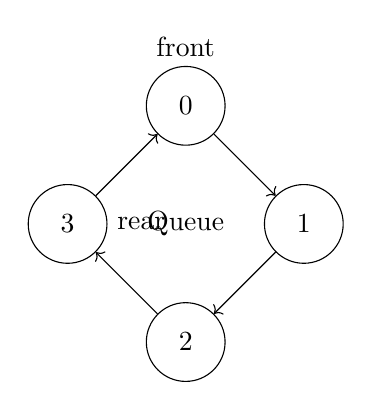
\begin{tikzpicture}
    \foreach \i in {0,1,2,3} {
        \node[draw, circle, minimum size=1cm] (n\i) at ({90-90*\i}:1.5) {\i};
    }
    \draw[->] (n0) -- (n1);
    \draw[->] (n1) -- (n2);
    \draw[->] (n2) -- (n3);
    \draw[->] (n3) -- (n0);
    
    \node at (0,0) {Queue};
    \node[above] at (n0.north) {front};
    \node[right] at (n3.east) {rear};
\end{tikzpicture}
\captionof{figure}{Circular Queue}
\end{center}

\textbf{INSERT Operation:}

\begin{enumerate}
    \item Check if queue is full
    \item If not full, increment rear
    \item If rear exceeds size, set rear = 0
    \item Insert element at rear position
\end{enumerate}

\textbf{DELETE Operation:}

\begin{enumerate}
    \item Check if queue is empty
    \item If not empty, remove element from front
    \item Increment front
    \item If front exceeds size, set front = 0
\end{enumerate}

\begin{itemize}
    \item \keyword{Circular nature}: Efficient memory utilization
    \item \keyword{No shifting}: Elements remain in place
    \item \keyword{Front-rear pointers}: Track queue boundaries
\end{itemize}
\end{solutionbox}

\begin{mnemonicbox}
Circular Saves Space
\end{mnemonicbox}

\questionmarks{2(a OR)}{3}{List out different Data Structure with examples.}

\begin{solutionbox}
\textbf{Answer}:

\begin{center}
\captionof{table}{Data Structure Types}
\begin{tabulary}{\linewidth}{|L|L|L|}
\hline
\textbf{Type} & \textbf{Data Structure} & \textbf{Example} \\
\hline
\textbf{Linear} & Array & [1,2,3,4] \\
\hline
\textbf{Linear} & Stack & Function calls \\
\hline
\textbf{Linear} & Queue & Printer queue \\
\hline
\textbf{Non-Linear} & Tree & File system \\
\hline
\textbf{Non-Linear} & Graph & Social network \\
\hline
\end{tabulary}
\end{center}
\end{solutionbox}

\begin{mnemonicbox}
Arrays-Stacks-Queues = Linear, Trees-Graphs = Non-linear
\end{mnemonicbox}

\questionmarks{2(b OR)}{4}{Discuss how the concept of circular queue is different from simple queue.}

\begin{solutionbox}
\textbf{Answer}:

\begin{center}
\captionof{table}{Simple vs Circular Queue}
\begin{tabulary}{\linewidth}{|L|L|}
\hline
\textbf{Simple Queue} & \textbf{Circular Queue} \\
\hline
Linear arrangement & Circular arrangement \\
\hline
Memory wastage & Efficient memory use \\
\hline
Fixed front and rear & Wraparound pointers \\
\hline
False overflow & True overflow detection \\
\hline
\end{tabulary}
\end{center}

\begin{itemize}
    \item \keyword{Memory efficiency}: Circular reuses deleted spaces
    \item \keyword{Pointer management}: Modulo arithmetic for wraparound
    \item \keyword{Performance}: Better space utilization
\end{itemize}
\end{solutionbox}

\begin{mnemonicbox}
Circular Conquers memory problems
\end{mnemonicbox}

\questionmarks{2(c OR)}{7}{Define stack. Explain PUSH \& POP operation with example. Write an algorithm for PUSH and POP operations of stack.}

\begin{solutionbox}
\textbf{Answer}:

\keyword{Stack}: LIFO (Last In First Out) data structure.

\textbf{PUSH Algorithm:}

\begin{enumerate}
    \item Check if stack is full
    \item If not full, increment top
    \item Insert element at top position
    \item Update top pointer
\end{enumerate}

\textbf{POP Algorithm:}

\begin{enumerate}
    \item Check if stack is empty
    \item If not empty, store top element
    \item Decrement top pointer
    \item Return stored element
\end{enumerate}

\textbf{Example:}

\begin{lstlisting}[language=Python,caption={Stack Example}]
Stack: [10, 20, 30] <- top
PUSH 40: [10, 20, 30, 40] <- top
POP: returns 40, stack: [10, 20, 30] <- top
\end{lstlisting}

\begin{itemize}
    \item \keyword{LIFO principle}: Last element added is first removed
    \item \keyword{Top pointer}: Tracks current stack position
    \item \keyword{Overflow/Underflow}: Check before operations
\end{itemize}
\end{solutionbox}

\begin{mnemonicbox}
Stack Stores in Last-in-first-out
\end{mnemonicbox}

\questionmarks{3(a)}{3}{Convert following infix expression to postfix: ( ( ( A - B ) * C ) + ( ( D - E ) / F ) )}

\begin{solutionbox}
\textbf{Answer}:

\textbf{Step-by-step conversion:}

\begin{center}
\captionof{table}{Infix to Postfix Conversion}
\begin{tabulary}{\linewidth}{|C|L|L|L|}
\hline
\textbf{Step} & \textbf{Scanned} & \textbf{Stack} & \textbf{Postfix} \\
\hline
1 & ( & ( & \\
\hline
2 & ( & (( & \\
\hline
3 & ( & ((( & \\
\hline
4 & A & ((( & A \\
\hline
5 & - & (((- & A \\
\hline
6 & B & (((- & AB \\
\hline
7 & ) & (( & AB- \\
\hline
8 & * & ((* & AB- \\
\hline
9 & C & ((* & AB-C \\
\hline
10 & ) & ( & AB-C* \\
\hline
11 & + & (+ & AB-C* \\
\hline
12 & ( & (+( & AB-C* \\
\hline
13 & ( & (+(( & AB-C* \\
\hline
14 & D & (+(( & AB-C*D \\
\hline
15 & - & (+((- & AB-C*D \\
\hline
16 & E & (+((- & AB-C*DE \\
\hline
17 & ) & (+ & AB-C*DE- \\
\hline
18 & / & (+(/ & AB-C*DE- \\
\hline
19 & F & (+(/ & AB-C*DE-F \\
\hline
20 & ) & (+ & AB-C*DE-F/ \\
\hline
21 & ) & & AB-C*DE-F/+ \\
\hline
\end{tabulary}
\end{center}

\textbf{Final Answer: AB-C*DE-F/+}
\end{solutionbox}

\begin{mnemonicbox}
Postfix Places operators after operands
\end{mnemonicbox}

\questionmarks{3(b)}{4}{Write a short note on doubly linked list.}

\begin{solutionbox}
\textbf{Answer}:

\keyword{Doubly Linked List}: Linear data structure with bidirectional links.

\textbf{Structure:}

\begin{center}
\begin{tikzpicture}[gtu box]
    \node (null1) at (-2,0) {NULL};
    \node[draw, rectangle split, rectangle split parts=3, rectangle split horizontal] (n1) at (0,0) {prev \nodepart{second} data \nodepart{third} next};
    \node[draw, rectangle split, rectangle split parts=3, rectangle split horizontal] (n2) at (3,0) {prev \nodepart{second} data \nodepart{third} next};
    \node[draw, rectangle split, rectangle split parts=3, rectangle split horizontal] (n3) at (6,0) {prev \nodepart{second} data \nodepart{third} next};
    \node (null2) at (8,0) {NULL};

    \draw[->] (null1) -- (n1);
    \draw[->] (n1.three) -- (n2.one);
    \draw[->] (n2.one) -- (n1.three);
    \draw[->] (n2.three) -- (n3.one);
    \draw[->] (n3.one) -- (n2.three);
    \draw[->] (n3.three) -- (null2);
\end{tikzpicture}
\captionof{figure}{Doubly Linked List}
\end{center}

\textbf{Advantages:}

\begin{itemize}
    \item \keyword{Bidirectional traversal}: Forward and backward navigation
    \item \keyword{Efficient deletion}: No need for previous node reference
    \item \keyword{Better insertion}: Can insert before given node easily
\end{itemize}

\textbf{Disadvantages:}

\begin{itemize}
    \item \keyword{Extra memory}: Additional pointer storage
    \item \keyword{Complex operations}: More pointer manipulations
\end{itemize}
\end{solutionbox}

\begin{mnemonicbox}
Doubly Delivers Bidirectional Benefits
\end{mnemonicbox}

\questionmarks{3(c)}{7}{Write a Python Program to delete first and last node from singly linked list.}

\begin{solutionbox}
\textbf{Answer}:

\textbf{Code:}

\begin{lstlisting}[language=Python,caption={Singly Linked List Deletion}]
class Node:
    def __init__(self, data):
        self.data = data
        self.next = None

class LinkedList:
    def __init__(self):
        self.head = None
    
    def delete_first(self):
        if self.head is None:
            return "List is empty"
        self.head = self.head.next
        return "First node deleted"
    
    def delete_last(self):
        if self.head is None:
            return "List is empty"
        if self.head.next is None:
            self.head = None
            return "Last node deleted"
        
        current = self.head
        while current.next.next:
            current = current.next
        current.next = None
        return "Last node deleted"
    
    def display(self):
        elements = []
        current = self.head
        while current:
            elements.append(current.data)
            current = current.next
        return elements

# Usage
ll = LinkedList()
# Add nodes and test deletion
\end{lstlisting}

\begin{itemize}
    \item \keyword{Delete first}: Update head pointer
    \item \keyword{Delete last}: Traverse to second last node
    \item \keyword{Edge cases}: Empty list and single node
\end{itemize}
\end{solutionbox}

\begin{mnemonicbox}
Delete Delivers by pointer updates
\end{mnemonicbox}

\questionmarks{3(a OR)}{3}{List different applications of Queue.}

\begin{solutionbox}
\textbf{Answer}:

\textbf{Queue Applications:}

\begin{center}
\captionof{table}{Queue Applications}
\begin{tabulary}{\linewidth}{|L|L|}
\hline
\textbf{Application} & \textbf{Usage} \\
\hline
\textbf{CPU Scheduling} & Process management \\
\hline
\textbf{Print Queue} & Document printing \\
\hline
\textbf{BFS Algorithm} & Graph traversal \\
\hline
\textbf{Buffer} & Data streaming \\
\hline
\end{tabulary}
\end{center}

\begin{itemize}
    \item \keyword{FIFO nature}: First come first served
    \item \keyword{Real-time systems}: Handle requests in order
    \item \keyword{Resource sharing}: Fair allocation
\end{itemize}
\end{solutionbox}

\begin{mnemonicbox}
Queues Quietly handle ordered operations
\end{mnemonicbox}

\questionmarks{3(b OR)}{4}{Explain different operations which we can perform on singly linked list.}

\begin{solutionbox}
\textbf{Answer}:

\textbf{Singly Linked List Operations:}

\begin{center}
\captionof{table}{Singly Linked List Operations}
\begin{tabulary}{\linewidth}{|L|L|}
\hline
\textbf{Operation} & \textbf{Description} \\
\hline
\textbf{Insertion} & Add node at beginning/end/middle \\
\hline
\textbf{Deletion} & Remove node from any position \\
\hline
\textbf{Traversal} & Visit all nodes sequentially \\
\hline
\textbf{Search} & Find specific data in list \\
\hline
\textbf{Count} & Count total number of nodes \\
\hline
\end{tabulary}
\end{center}

\begin{itemize}
    \item \keyword{Dynamic size}: Grow/shrink during runtime
    \item \keyword{Memory efficiency}: Allocate as needed
    \item \keyword{Sequential access}: No random access
\end{itemize}
\end{solutionbox}

\begin{mnemonicbox}
Insert-Delete-Traverse-Search-Count
\end{mnemonicbox}

\questionmarks{3(c OR)}{7}{Write an algorithm to insert a new node at the end of doubly linked list.}

\begin{solutionbox}
\textbf{Answer}:

\textbf{Algorithm for insertion at end:}

\begin{enumerate}
    \item Create new node with given data
    \item Set new node's next = NULL
    \item If list is empty:
    \begin{itemize}
        \item Set head = new node
        \item Set new node's prev = NULL
    \end{itemize}
    \item Else:
    \begin{itemize}
        \item Traverse to last node
        \item Set last node's next = new node
        \item Set new node's prev = last node
    \end{itemize}
    \item Return success
\end{enumerate}

\textbf{Code:}

\begin{lstlisting}[language=Python,caption={Insert at End Doubly Linked List}]
def insert_at_end(self, data):
    new_node = Node(data)
    if self.head is None:
        self.head = new_node
        return
    
    current = self.head
    while current.next:
        current = current.next
    
    current.next = new_node
    new_node.prev = current
\end{lstlisting}

\begin{itemize}
    \item \keyword{Two-way linking}: Update both next and prev pointers
    \item \keyword{End insertion}: Traverse to find last node
    \item \keyword{Bidirectional connection}: Maintain list integrity
\end{itemize}
\end{solutionbox}

\begin{mnemonicbox}
Insert Intelligently with bidirectional links
\end{mnemonicbox}

\questionmarks{4(a)}{3}{Write a python program for linear search.}

\begin{solutionbox}
\textbf{Answer}:

\textbf{Code:}

\begin{lstlisting}[language=Python,caption={Linear Search}]
def linear_search(arr, target):
    for i in range(len(arr)):
        if arr[i] == target:
            return i
    return -1

# Example usage
data = [10, 20, 30, 40, 50]
result = linear_search(data, 30)
print(f"Element found at index: {result}")
\end{lstlisting}

\begin{itemize}
    \item \keyword{Sequential search}: Check each element one by one
    \item \keyword{Time complexity}: O(n)
    \item \keyword{Simple implementation}: Easy to understand
\end{itemize}
\end{solutionbox}

\begin{mnemonicbox}
Linear Looks through every element
\end{mnemonicbox}

\questionmarks{4(b)}{4}{Write a short note on Circular linked list.}

\begin{solutionbox}
\textbf{Answer}:

\keyword{Circular Linked List}: Last node points back to first node forming a circle.

\textbf{Diagram:}

\begin{center}
\begin{tikzpicture}[gtu box]
    \node[draw, rectangle split, rectangle split parts=2, rectangle split horizontal] (n1) at (0,0) {data \nodepart{second} next};
    \node[draw, rectangle split, rectangle split parts=2, rectangle split horizontal] (n2) at (3,0) {data \nodepart{second} next};
    \node[draw, rectangle split, rectangle split parts=2, rectangle split horizontal] (n3) at (6,0) {data \nodepart{second} next};

    \draw[->] (n1.second) -- (n2);
    \draw[->] (n2.second) -- (n3);
    \draw[->] (n3.second) -- ++(0,-0.7) -| (n1);
\end{tikzpicture}
\captionof{figure}{Circular Linked List}
\end{center}

\textbf{Characteristics:}

\begin{itemize}
    \item \keyword{No NULL pointers}: Last node connects to first
    \item \keyword{Continuous traversal}: Can traverse infinitely
    \item \keyword{Memory efficiency}: Better cache performance
    \item \keyword{Applications}: Round-robin scheduling, multiplayer games
\end{itemize}

\textbf{Advantages:}

\begin{itemize}
    \item \keyword{Efficient insertion}: At any position
    \item \keyword{No wasted pointers}: All nodes connected
\end{itemize}
\end{solutionbox}

\begin{mnemonicbox}
Circular Connects everything in a loop
\end{mnemonicbox}

\questionmarks{4(c)}{7}{Explain Quick sort algorithm with an example.}

\begin{solutionbox}
\textbf{Answer}:

\keyword{Quick Sort}: Divide and conquer sorting algorithm using pivot element.

\textbf{Algorithm:}

\begin{enumerate}
    \item Choose pivot element
    \item Partition array around pivot
    \item Recursively sort left subarray
    \item Recursively sort right subarray
\end{enumerate}

\textbf{Example: Sort [64, 34, 25, 12, 22, 11, 90]}

\textbf{Step 1:} Pivot = 64

\begin{center}
\code{[34, 25, 12, 22, 11] 64 [90]}
\end{center}

\textbf{Step 2:} Sort left partition [34, 25, 12, 22, 11] (Pivot = 34)

\begin{center}
\code{[25, 12, 22, 11] 34 []}
\end{center}

\textbf{Final sorted:} [11, 12, 22, 25, 34, 64, 90]

\begin{itemize}
    \item \keyword{Divide and conquer}: Break problem into smaller parts
    \item \keyword{In-place sorting}: Minimal extra memory
    \item \keyword{Average complexity}: O(n log n)
\end{itemize}
\end{solutionbox}

\begin{mnemonicbox}
Quick Partitions then conquers
\end{mnemonicbox}

\questionmarks{4(a OR)}{3}{Explain Binary search algorithm with an example.}

\begin{solutionbox}
\textbf{Answer}:

\keyword{Binary Search}: Search algorithm for sorted arrays using divide and conquer.

\textbf{Algorithm:}

\begin{enumerate}
    \item Set left = 0, right = array length - 1
    \item While left <= right:
    \begin{itemize}
        \item Calculate mid = (left + right) / 2
        \item If target = array[mid], return mid
        \item If target $<$ array[mid], right = mid - 1
        \item If target $>$ array[mid], left = mid + 1
    \end{itemize}
    \item Return -1 if not found
\end{enumerate}

\textbf{Example: Search 22 in [11, 12, 22, 25, 34, 64, 90]}

\begin{center}
\captionof{table}{Binary Search Trace}
\begin{tabulary}{\linewidth}{|C|C|C|C|C|L|}
\hline
\textbf{Step} & \textbf{Left} & \textbf{Right} & \textbf{Mid} & \textbf{Value} & \textbf{Action} \\
\hline
1 & 0 & 6 & 3 & 25 & 22 $<$ 25, right = 2 \\
\hline
2 & 0 & 2 & 1 & 12 & 22 $>$ 12, left = 2 \\
\hline
3 & 2 & 2 & 2 & 22 & Found! \\
\hline
\end{tabulary}
\end{center}
\end{solutionbox}

\begin{mnemonicbox}
Binary Bisects to find quickly
\end{mnemonicbox}

\questionmarks{4(b OR)}{4}{Discuss different applications of linked list.}

\begin{solutionbox}
\textbf{Answer}:

\textbf{Linked List Applications:}

\begin{center}
\captionof{table}{Linked List Applications}
\begin{tabulary}{\linewidth}{|L|L|}
\hline
\textbf{Application} & \textbf{Usage} \\
\hline
\textbf{Dynamic Arrays} & Resizable data storage \\
\hline
\textbf{Stack/Queue Implementation} & LIFO/FIFO structures \\
\hline
\textbf{Graph Representation} & Adjacency lists \\
\hline
\textbf{Memory Management} & Free memory blocks \\
\hline
\textbf{Music Playlist} & Next/previous song navigation \\
\hline
\end{tabulary}
\end{center}

\begin{itemize}
    \item \keyword{Dynamic memory}: Allocate as needed
    \item \keyword{Efficient insertion/deletion}: No shifting required
    \item \keyword{Flexible structure}: Adapt to changing requirements
\end{itemize}
\end{solutionbox}

\begin{mnemonicbox}
Linked Lists Live in dynamic applications
\end{mnemonicbox}

\questionmarks{4(c OR)}{7}{Write a python program for insertion sort with an example.}

\begin{solutionbox}
\textbf{Answer}:

\textbf{Code:}

\begin{lstlisting}[language=Python,caption={Insertion Sort}]
def insertion_sort(arr):
    for i in range(1, len(arr)):
        key = arr[i]
        j = i - 1
        
        while j >= 0 and arr[j] > key:
            arr[j + 1] = arr[j]
            j -= 1
        
        arr[j + 1] = key
    
    return arr

# Example
data = [64, 34, 25, 12, 22, 11, 90]
sorted_data = insertion_sort(data)
print(f"Sorted array: {sorted_data}")
\end{lstlisting}

\textbf{Step-by-step example:}

\begin{itemize}
    \item Initial: [64, 34, 25, 12, 22, 11, 90]
    \item Pass 1:  [34, 64, 25, 12, 22, 11, 90]
    \item Pass 2:  [25, 34, 64, 12, 22, 11, 90]
    \item Pass 3:  [12, 25, 34, 64, 22, 11, 90]
    \item Pass 4:  [12, 22, 25, 34, 64, 11, 90]
    \item Pass 5:  [11, 12, 22, 25, 34, 64, 90]
    \item Pass 6:  [11, 12, 22, 25, 34, 64, 90]
\end{itemize}

\begin{itemize}
    \item \keyword{Card sorting analogy}: Like arranging playing cards
    \item \keyword{Stable sort}: Maintains relative order of equal elements
    \item \keyword{Online algorithm}: Can sort list as it receives data
\end{itemize}
\end{solutionbox}

\begin{mnemonicbox}
Insertion Inserts in right position
\end{mnemonicbox}

\questionmarks{5(a)}{3}{Define following terms: I. Complete Binary tree II. In-degree III. Out-degree.}

\begin{solutionbox}
\textbf{Answer}:

\begin{center}
\captionof{table}{Binary Tree Terms}
\begin{tabulary}{\linewidth}{|L|L|}
\hline
\textbf{Term} & \textbf{Definition} \\
\hline
\textbf{Complete Binary Tree} & All levels filled except possibly last level from left \\
\hline
\textbf{In-degree} & Number of edges coming into a node \\
\hline
\textbf{Out-degree} & Number of edges going out from a node \\
\hline
\end{tabulary}
\end{center}
\end{solutionbox}

\begin{mnemonicbox}
Complete-In-Out = Tree terminology
\end{mnemonicbox}

\questionmarks{5(b)}{4}{Explain bubble sort algorithm with an example.}

\begin{solutionbox}
\textbf{Answer}:

\keyword{Bubble Sort}: Compare adjacent elements and swap if in wrong order.

\textbf{Algorithm:}

\begin{enumerate}
    \item For each pass (0 to n-1):
    \item For each element (0 to n-pass-1):
    \item If arr[j] $>$ arr[j+1]:
    \item Swap arr[j] and arr[j+1]
\end{enumerate}

\textbf{Example: [64, 34, 25, 12]}

\begin{center}
\captionof{table}{Bubble Sort Trace}
\begin{tabulary}{\linewidth}{|L|L|L|}
\hline
\textbf{Pass} & \textbf{Comparisons} & \textbf{Result} \\
\hline
1 & 64$>$34(swap), 64$>$25(swap), 64$>$12(swap) & [34,25,12,64] \\
\hline
2 & 34$>$25(swap), 34$>$12(swap) & [25,12,34,64] \\
\hline
3 & 25$>$12(swap) & [12,25,34,64] \\
\hline
\end{tabulary}
\end{center}

\begin{itemize}
    \item \keyword{Bubble up}: Largest element bubbles to end
    \item \keyword{Multiple passes}: Each pass places one element correctly
    \item \keyword{Simple implementation}: Easy to understand
\end{itemize}
\end{solutionbox}

\begin{mnemonicbox}
Bubble Brings biggest to back
\end{mnemonicbox}

\questionmarks{5(c)}{7}{Create a Binary Search Tree for the keys 15, 35, 12, 48, 5, 25, 58, 8 and write the Preorder, Inorder and Postorder traversal sequences.}

\begin{solutionbox}
\textbf{Answer}:

\textbf{BST Construction:}

\begin{center}
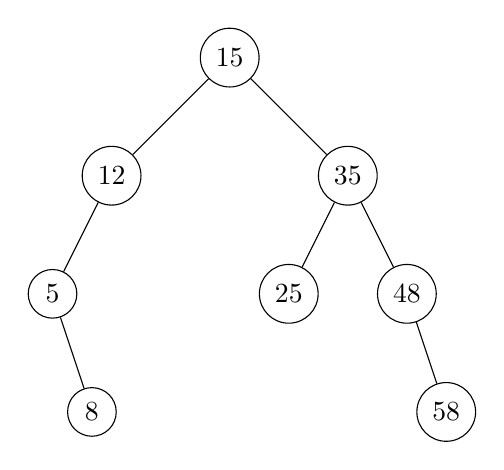
\begin{tikzpicture}[
    level 1/.style={sibling distance=3cm},
    level 2/.style={sibling distance=1.5cm},
    level 3/.style={sibling distance=1cm}]
    
    \node[circle, draw] {15}
        child {node[circle, draw] {12}
            child {node[circle, draw] {5}
                child[missing]
                child {node[circle, draw] {8}}
            }
            child[missing]
        }
        child {node[circle, draw] {35}
            child {node[circle, draw] {25}}
            child {node[circle, draw] {48}
                child[missing]
                child {node[circle, draw] {58}}
            }
        };
\end{tikzpicture}
\captionof{figure}{Binary Search Tree}
\end{center}

\textbf{Traversal Sequences:}

\begin{center}
\captionof{table}{Traversals}
\begin{tabulary}{\linewidth}{|L|L|}
\hline
\textbf{Traversal} & \textbf{Sequence} \\
\hline
\textbf{Preorder} & 15, 12, 5, 8, 35, 25, 48, 58 \\
\hline
\textbf{Inorder} & 5, 8, 12, 15, 25, 35, 48, 58 \\
\hline
\textbf{Postorder} & 8, 5, 12, 25, 58, 48, 35, 15 \\
\hline
\end{tabulary}
\end{center}

\textbf{Traversal Rules:}

\begin{itemize}
    \item \keyword{Preorder}: Root $\rightarrow$ Left $\rightarrow$ Right
    \item \keyword{Inorder}: Left $\rightarrow$ Root $\rightarrow$ Right (gives sorted order)
    \item \keyword{Postorder}: Left $\rightarrow$ Right $\rightarrow$ Root
\end{itemize}
\end{solutionbox}

\begin{mnemonicbox}
Pre-In-Post = Root position
\end{mnemonicbox}

\questionmarks{5(a OR)}{3}{Define binary tree. Explain searching a node in binary tree.}

\begin{solutionbox}
\textbf{Answer}:

\keyword{Binary Tree}: Hierarchical data structure where each node has at most two children.

\textbf{Search Algorithm:}

\begin{enumerate}
    \item Start from root
    \item If target = current node, return found
    \item If target $<$ current node, go left
    \item If target $>$ current node, go right
    \item Repeat until found or reach NULL
\end{enumerate}

\begin{itemize}
    \item \keyword{Hierarchical structure}: Parent-child relationship
    \item \keyword{Binary property}: Maximum two children per node
    \item \keyword{Search efficiency}: O(log n) for balanced trees
\end{itemize}
\end{solutionbox}

\begin{mnemonicbox}
Binary Branches into two paths
\end{mnemonicbox}

\questionmarks{5(b OR)}{4}{Give the trace to sort the given data using bubble sort method. Data are: 44, 72, 94, 28, 18, 442, 41}

\begin{solutionbox}
\textbf{Answer}:

\textbf{Bubble Sort Trace:}

\begin{center}
\captionof{table}{Bubble Sort Trace}
\begin{tabulary}{\linewidth}{|L|L|L|}
\hline
\textbf{Pass} & \textbf{Array State} & \textbf{Swaps} \\
\hline
Initial & [44, 72, 94, 28, 18, 442, 41] & - \\
\hline
Pass 1 & [44, 72, 28, 18, 94, 41, 442] & 94$>$28, 94$>$18, 442$>$41 \\
\hline
Pass 2 & [44, 28, 18, 72, 41, 94, 442] & 72$>$28, 72$>$18, 94$>$41 \\
\hline
Pass 3 & [28, 18, 44, 41, 72, 94, 442] & 44$>$28, 44$>$18, 72$>$41 \\
\hline
Pass 4 & [18, 28, 41, 44, 72, 94, 442] & 28$>$18, 44$>$41 \\
\hline
Pass 5 & [18, 28, 41, 44, 72, 94, 442] & No swaps \\
\hline
\end{tabulary}
\end{center}

\textbf{Final sorted array:} [18, 28, 41, 44, 72, 94, 442]
\end{solutionbox}

\begin{mnemonicbox}
Bubble sort Bubbles largest to end each pass
\end{mnemonicbox}

\questionmarks{5(c OR)}{7}{List applications of trees. Explain the technique for converting general tree into a Binary Search Tree with example.}

\begin{solutionbox}
\textbf{Answer}:

\textbf{Tree Applications:}

\begin{center}
\captionof{table}{Tree Applications}
\begin{tabulary}{\linewidth}{|L|L|}
\hline
\textbf{Application} & \textbf{Usage} \\
\hline
\textbf{File System} & Directory hierarchy \\
\hline
\textbf{Expression Trees} & Mathematical expressions \\
\hline
\textbf{Decision Trees} & AI and machine learning \\
\hline
\textbf{Heap} & Priority queues \\
\hline
\end{tabulary}
\end{center}

\textbf{General Tree to BST Conversion:}

\textbf{Technique: First Child - Next Sibling Representation}

\textbf{Original General Tree:}

\begin{center}
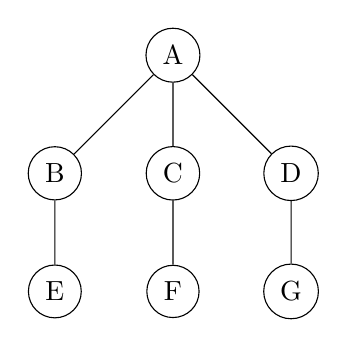
\begin{tikzpicture}
    \node[circle, draw] {A}
        child {node[circle, draw] {B}
            child {node[circle, draw] {E}}
        }
        child {node[circle, draw] {C}
            child {node[circle, draw] {F}}
        }
        child {node[circle, draw] {D}
            child {node[circle, draw] {G}}
        };
\end{tikzpicture}
\captionof{figure}{General Tree}
\end{center}

\textbf{Converted to Binary Tree:}

\begin{center}
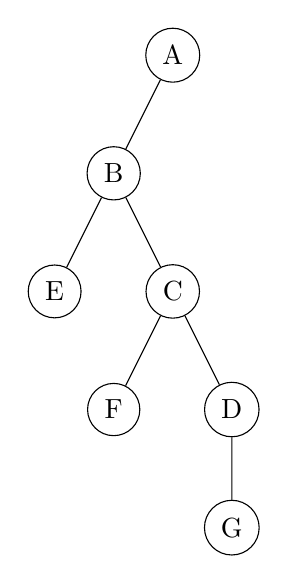
\begin{tikzpicture}
    \node[circle, draw] {A}
        child {node[circle, draw] {B}
            child {node[circle, draw] {E}}
            child {node[circle, draw] {C}
                child {node[circle, draw] {F}}
                child {node[circle, draw] {D}
                    child {node[circle, draw] {G}}
                }
            }
        }
        child[missing];
\end{tikzpicture}
\captionof{figure}{Converted Binary Tree}
\end{center}

\textbf{Steps:}

\begin{enumerate}
    \item \keyword{First child}: Becomes left child in binary tree
    \item \keyword{Next sibling}: Becomes right child in binary tree
    \item \keyword{Recursive application}: Apply to all nodes
\end{enumerate}

\begin{itemize}
    \item \keyword{Systematic conversion}: Preserves tree structure
    \item \keyword{Binary representation}: Uses only two pointers per node
    \item \keyword{Space efficiency}: Standard binary tree operations apply
\end{itemize}
\end{solutionbox}

\begin{mnemonicbox}
First-child Left, Next-sibling Right
\end{mnemonicbox}

\end{document}
